\vspace{-8cm}
\section{Tablas análisis de datos}

\begin{table}[h]
    \centering
    \caption{Instancias Operativas AM/PM}
    \label{tab:instancias operativas}
    \vspace{0.5em}
    % El @{\extracolsep{\fill}} hace que LaTeX calcule el espacio entre columnas solo
    \begin{tabular*}{\textwidth}{@{\extracolsep{\fill}} l l l @{}}
        \toprule
        \textbf{Característica} & \textbf{AM (mañana)} & \textbf{PM (tarde/noche)} \\ \midrule
        Archivo & AM\_large.xlsx & PM\_small.xlsx \\ \addlinespace
        Fecha de operación & 31 de marzo 2026 & 26--27 de marzo 2026 \\ \addlinespace
        Nº de pasajeros & \textbf{620} & \textbf{347} \\ \addlinespace
        Domicilios únicos & 604 & 341 \\ \addlinespace
        Centros de trabajo únicos & 36 & 26 \\ \bottomrule
    \end{tabular*}
\end{table}



\begin{table}[h]
    \centering
    \caption{Distribución por Prioridad AM/PM}
    \label{tab:distribucion por prioridad}
    \vspace{0.5em}
    \begin{tabular*}{\textwidth}{@{\extracolsep{\fill}} l r r @{}}
        \toprule
        \textbf{Prioridad} & \textbf{AM — n (\%)} & \textbf{PM — n (\%)} \\ \midrule
        1 (más alta) & 88 (14,2 \%) & 66 (19,0 \%) \\ \addlinespace
        2            & 218 (35,2 \%) & 123 (35,4 \%) \\ \addlinespace
        3            & 280 (45,2 \%) & 142 (40,9 \%) \\ \addlinespace
        4 (más baja) & 34 (5,5 \%)  & 16 (4,6 \%) \\ \bottomrule
    \end{tabular*}
\end{table}

\begin{table}[h]
    \centering
    \caption{Tiempos Máximos de Espera y en Vehículo por Prioridad}
    \label{tab:tiempos de espera y en vehi}
    \vspace{0.5em}
    \begin{tabular*}{\textwidth}{@{\extracolsep{\fill}} l r r @{}}
        \toprule
        \textbf{Prioridad} & \textbf{Tiempo máx. espera (min)} & \textbf{Tiempo máx. en vehículo (min)} \\ \midrule
        1 & 40 & 80 \\ \addlinespace
        2 & 20 & 60 \\ \addlinespace
        3 & 15 & 60 \\ \addlinespace
        4 & 5  & 50 \\ \bottomrule
    \end{tabular*}
\end{table}


\begin{table}[h]
    \centering
    \caption{Flota de vehículos}
    \label{tab:flota de vehi}
    \vspace{0.5em}
    \begin{tabular*}{\textwidth}{@{\extracolsep{\fill}} l r r r @{}}
        \toprule
        \textbf{Tipo} & \textbf{Capacidad (asientos)} & \textbf{Stock disponible} & \textbf{Costo fijo (CLP)} \\ \midrule
        Common & 3 & 500 & 2.200 \\ \addlinespace
        Large  & 6 & 50  & 4.500 \\ \bottomrule
    \end{tabular*}
\end{table}


\begin{table}[h]
    \centering
    \caption{Variación de tiempos de viaje según la hora}
    \label{tab:var de tiempos}
    \vspace{0.5em}
    \begin{tabular*}{\textwidth}{@{\extracolsep{\fill}} l r r l @{}}
        \toprule
        \textbf{Hora} & \textbf{Tiempo medio (min)} & \textbf{Velocidad media (km/h)} & \textbf{Instancia} \\ \midrule
        04:00 & 25,1 & 38,8 & AM \\ \addlinespace
        05:00 & 25,3 & 38,5 & AM \\ \addlinespace
        06:00 & \textbf{26,3} & \textbf{37,1} & AM \\ \midrule
        22:00 & \textbf{28,6} & \textbf{33,9} & PM \\ \addlinespace
        23:00 & 25,6 & 37,7 & PM \\ \addlinespace
        00:00 & 24,8 & 38,9 & PM \\ \addlinespace
        01:00 & 24,8 & 38,9 & PM \\ \bottomrule
    \end{tabular*}
\end{table}

\begin{table}[h!]
    \centering
    \caption{Comparativa de Tiempos Pronosticados vs Reales}
    \label{tab:comparativa}
    \vspace{0.5em}
    \begin{tabular*}{\textwidth}{@{\extracolsep{\fill}} l r r @{}}
        \toprule
        \textbf{Métrica} & \textbf{Tiempo pronosticado (s)} & \textbf{Tiempo real (s)} \\ \midrule
        Media & 699,7 & 688,1 \\ \addlinespace
        Desviación estándar & 425,1 & 444,5 \\ \addlinespace
        Mínimo & 62,7 & 6,0 \\ \addlinespace
        Mediana & 610,2 & 593,0 \\ \addlinespace
        Máximo & 3.250,8 & 5.881,0 \\ \bottomrule
    \end{tabular*}
\end{table}

\clearpage
\section{Conjuntos y Parámetros del Modelo}
\label{anexo:conjuntos}
\subsection{Conjuntos}

\begin{itemize}
    \item $N = \{1,\dots,n\}$: solicitudes de transporte (pasajeros).
    \item $P = \{1,\dots,n\}$: nodos de recogida (\textit{pickup}), uno por solicitud.
    \item $D = \{n+1,\dots,2n\}$: nodos de entrega (\textit{delivery}). Para cada $i\in P$, su entrega asociada es $n+i\in D$.
    \item $V = P \cup D \cup \{0,\,2n+1\}$: conjunto total de nodos, con $0$ y $2n+1$ como depósitos virtuales de inicio y fin.
    \item $K$: flota de vehículos disponibles (cada $k\in K$ es un vehículo individual).
    \item $\mathcal{T} = \{\textsc{Common},\,\textsc{Large}\}$: tipos de vehículo, con $t(k)\in\mathcal{T}$ el tipo asignado a $k$.
    \item $R = \{1,2,3,4\}$: categorías sindicales.
    \item $\mathcal{A} = \{(r,r')\in R\times R : |r-r'|\leq 1\}$: pares de categorías compatibles (consecutivas).
\end{itemize}


\subsection{Parámetros}
\begin{itemize}
    \item $d_{ij}\in\mathbb{R}_+$: distancia (m) entre nodos $i$ y $j$.
    \item $\tau_{ij}(t)\in\mathbb{R}_+$: tiempo de viaje (s) entre $i$ y $j$ si se parte en el instante $t$; función escalonada por hora obtenida de las matrices horarias y afinada por el modelo XGBoost.
    \item $Q^{t(k)}\in\mathbb{Z}_+$: capacidad (asientos) del tipo $t(k)$; $Q^{\textsc{Common}}=3$, $Q^{\textsc{Large}}=6$.
    \item $F^{t(k)}\in\mathbb{R}_+$: costo fijo (CLP) por utilizar un vehículo de tipo $t(k)$; $F^{\textsc{Common}}=2\,200$, $F^{\textsc{Large}}=4\,500$.
    \item $c^{\mathrm{var}}=0{,}8$ CLP/m: costo variable por metro recorrido.
    \item $s_i\in\mathbb{R}_+$: tiempo de parada (s) en el nodo $i$: $s_i=180$ si $i\in P$; $s_i=60$ si $i\in D$; $s_0=s_{2n+1}=0$.
    \item $q_i\in\mathbb{Z}$: variación de carga al visitar el nodo $i$: $q_i=+1$ si $i\in P$; $q_i=-1$ si $i\in D$; $q_0=q_{2n+1}=0$.
    \item $r_i\in R$: categoría sindical del pasajero $i$.
    \item $\sigma_i\in\mathbb{R}_+$: hora de inicio de turno del pasajero $i$ (caso AM) u hora de fin de turno (caso PM).
    \item $e_i\in\mathbb{R}_+$: cota inferior de la ventana de tiempo en el nodo $i$.
    \item $l_i\in\mathbb{R}_+$: cota superior de la ventana de tiempo en el nodo $i$.
    \item $W_r\in\mathbb{R}_+$: tiempo máximo de espera/adelanto para la categoría $r$ (minutos).
    \item $M_r\in\mathbb{R}_+$: tiempo máximo en vehículo para la categoría $r$ (minutos).
    \item $M^\infty$: constante \textit{big-M} suficientemente grande.
\end{itemize}


\subsection{Variables de decisión}
\begin{itemize}
    \item $x_{ijk}\in\{0,1\}$: vale $1$ si el vehículo $k$ viaja directamente del nodo $i$ al $j$.
    \item $y_k\in\{0,1\}$: vale $1$ si el vehículo $k$ es utilizado.
    \item $B_{ik}\in\mathbb{R}_+$: instante en el que el vehículo $k$ inicia el servicio en el nodo $i$.
    \item $L_{ik}\in\mathbb{Z}_+$: carga a bordo de $k$ al salir de $i$.
    \item $u_{rk}\in\{0,1\}$: vale $1$ si el vehículo $k$ transporta al menos un pasajero de categoría $r$.
\end{itemize}

\subsection{Restricciones}
\vspace{-1cm}
\begin{align}
& \sum_{k\in K}\sum_{j\in V\setminus\{0\}} x_{ijk} = 1 && \forall i\in P \label{eq:r1}\\
& \sum_{j\in V} x_{ijk} \;-\; \sum_{j\in V} x_{j,\,n+i,\,k} = 0 && \forall i\in P,\; k\in K \label{eq:r2}\\
& \sum_{j\in V} x_{0jk} = y_k,\qquad \sum_{i\in V} x_{i,\,2n+1,\,k} = y_k && \forall k\in K \label{eq:r3}\\
& \sum_{i\in V} x_{ihk} \;-\; \sum_{j\in V} x_{hjk} = 0 && \forall h\in P\cup D,\; k\in K \label{eq:r4}\\
& B_{jk} \geq B_{ik} + s_i + \tau_{ij}(B_{ik}) - M^\infty(1-x_{ijk}) && \forall (i,j)\in V^2,\; k\in K \label{eq:r5}\\
& B_{ik} + s_i + \tau_{i,\,n+i}(B_{ik}) \leq B_{n+i,\,k} && \forall i\in P,\; k\in K \label{eq:r6}\\
& e_i \leq B_{ik} \leq l_i && \forall i\in V,\; k\in K \label{eq:r7}\\
& L_{jk} \geq L_{ik} + q_j - M^\infty(1-x_{ijk}) && \forall (i,j)\in V^2,\; k\in K \label{eq:r8}\\
& 0 \leq L_{ik} \leq Q^{t(k)} && \forall i\in V,\; k\in K \label{eq:r9}\\
& B_{n+i,k} - (B_{ik} + s_i) \leq M_{r_i} && \forall i\in P,\; k\in K \label{eq:r10}\\
& \sigma_i - (B_{n+i,k} + s_{n+i}) \leq W_{r_i} && \forall i\in P,\; k\in K \;(\mathrm{AM}) \label{eq:r11}\\
& u_{r_i,k} \geq \sum_{j\in V} x_{ijk} && \forall i\in P,\; k\in K \label{eq:r12}\\
& \sum_{r\in R} u_{rk} \leq 2 && \forall k\in K \label{eq:r13}\\
& u_{rk} + u_{r'k} \leq 1 && \forall k\in K,\; (r,r')\notin\mathcal{A} \label{eq:r14}
\end{align}



\clearpage
\section{Carta Gantt}
\begin{figure}[h] 
    \centering
    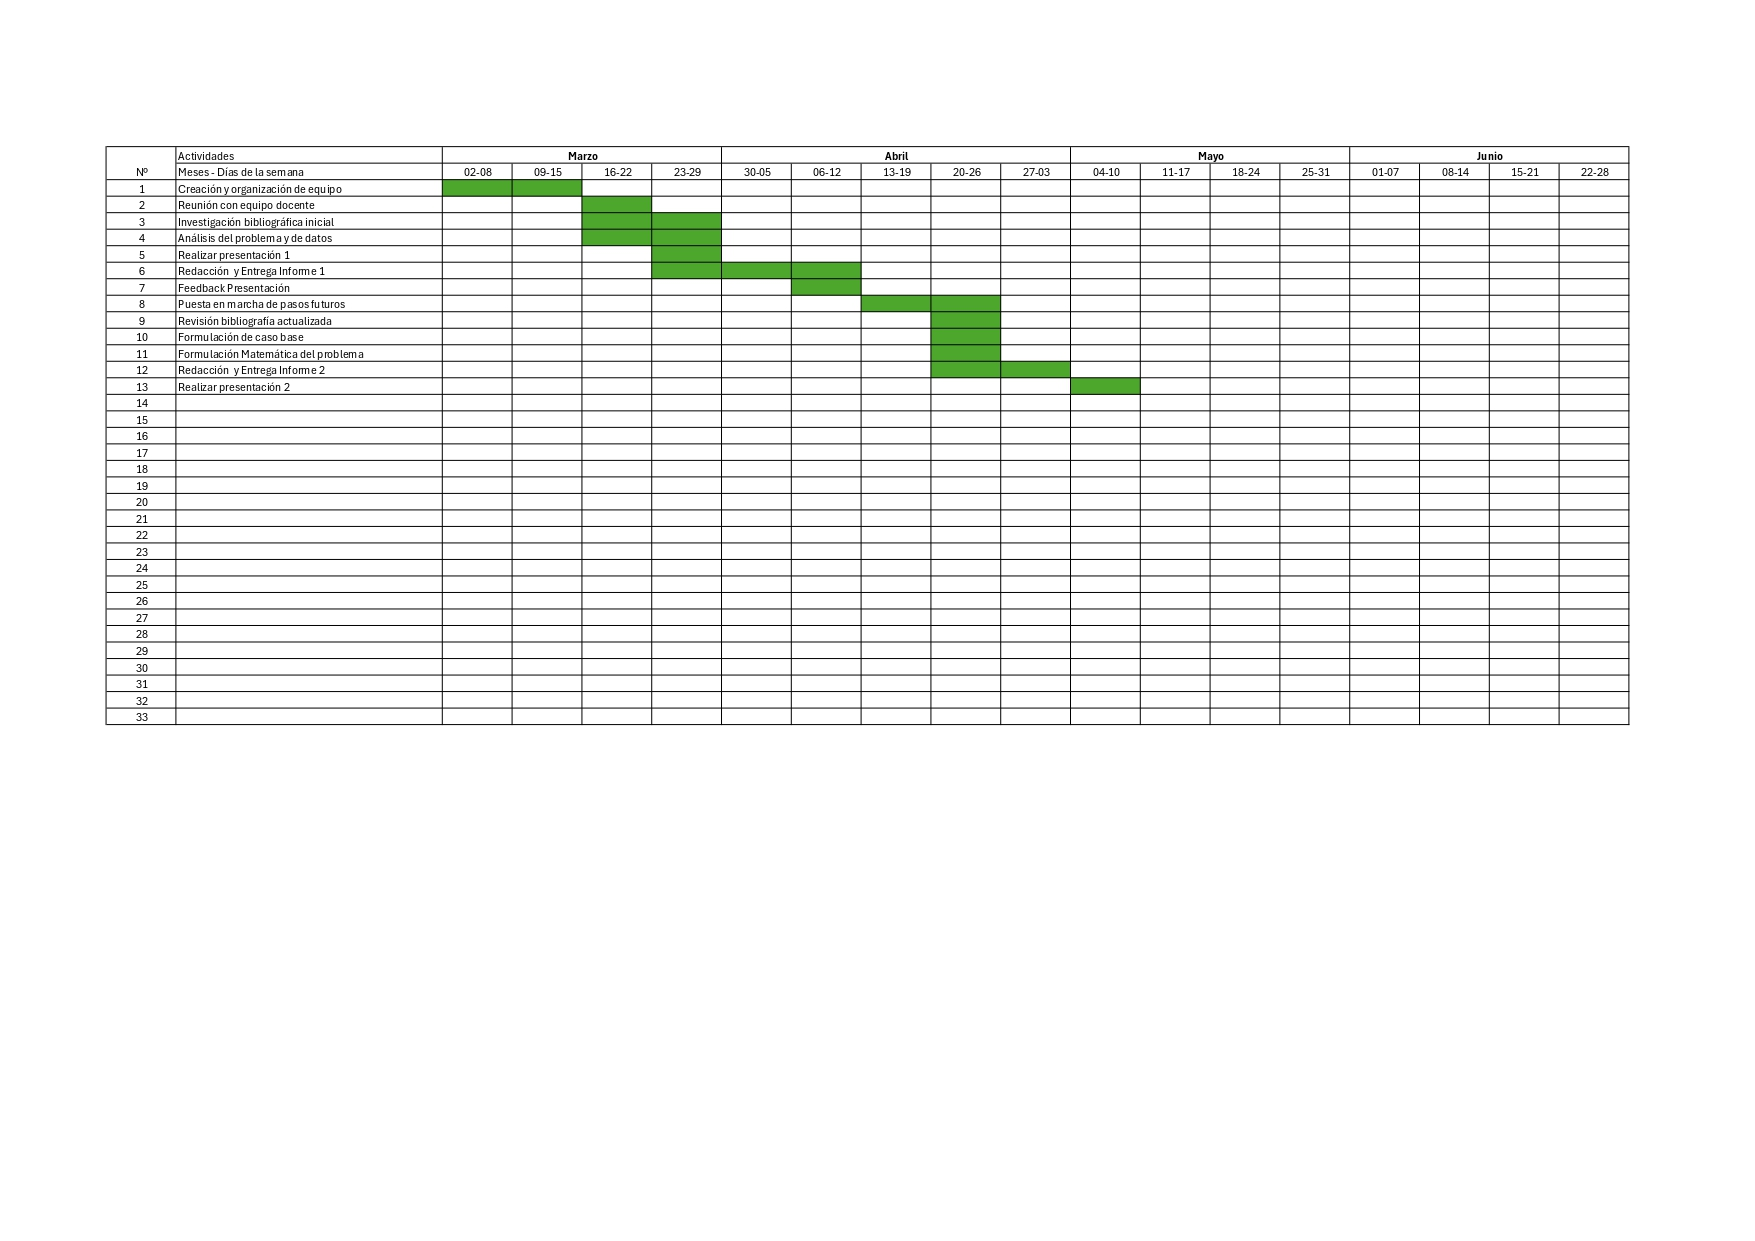
\includegraphics[width=1.2\textwidth, angle=90]{figures/Carta Gantt Capstone (1)_page-0001.jpg}
    \caption{Carta Gantt, Período Marzo-Mayo}
\end{figure}
